\subsection{Diseño Módulo 2}

En esta sección se establecen los fundamentos de las reglas que permiten 
clasificar automáticamente el estado del kéfir a partir de sus parámetros 
fisicoquímicos principales: pH, temperatura y concentración de $CO_{2}$. 
Con este propósito, se definen con precisión los rangos de cada variable, 
junto con sus respectivas etiquetas lingüísticas y funciones de pertenencia, 
las cuales han sido diseñadas considerando los márgenes de error típicos de los sensores 
especificados en la sección \ref{sec:mod1}.
Por consiguiente, este enfoque transforma las mediciones crudas en información cualitativa 
,creando las bases para una clasificación confiable del kéfir en 
categorías prácticas que orientan directamente la toma de decisiones del productor. 
A continuación, se describe detalladamente dicho proceso.

\subsubsection{Clasificación del kéfir}


En la fermentación del kéfir, las funciones de membresía permiten traducir 
la variabilidad metabólica de la glucólisis, la producción de $CO_2$ y 
la acidificación láctica en conjuntos difusos delimitados. Es fundamental definir
rangos operativos precisos para detectar oportunamente el intervalo ideal de recolección
(pH entre $4.2$ y $4.6$) y evitar la degradación hacia una fermentación acética indeseable. 
Para ello, se emplearán funciones de pertenencia trapezoidales, 
las cuales delimitan los umbrales críticos de temperatura, pH y generación de gas,
absorbiendo la dinámica no lineal e incierta de los microorganismos en cada lote.
\subsubsection{Tasa de acidificación}


Como primera parte para definir las clasificaciones del kéfir, 
se establecen los rangos del pH. Con base en la tabla \cref{tab:dominio_ph},
se especifican los rangos y las etiquetas lingüísticas que adopta el pH durante 
el proceso de fermentación del kéfir. Estos dominios, junto con sus respectivas 
funciones de pertenencia trapezoidales, la cual se define mediante la siguiente expresión matemática:

\begin{equation}
\mu(x) = 
\begin{cases}
0, & x \leq a \quad \vee \quad x \geq d \\[8pt]
\dfrac{x - a}{b - a}, & a \leq x \leq b \\[12pt]
1, & b \leq x \leq \\[12pt]
\dfrac{d - x}{d - c}, & c \leq x \leq d
\end{cases}
\label{eq:trapezoidal}
\end{equation}

donde \(a \leq b \leq c \leq d\) son los parámetros que delimitan la función.
Por lo que dicha función trapezoidal se ilustra en la \cref{fig:Log1}, 
donde se aprecia claramente la transición entre las categorías Óptimo, 
Adecuado, Subóptimo y Sobrefermentado.Asimismo para la selección de la función de pertenencia t
rapezoidal, se  tomo como base el módelo implementado en el proyecto \ref{sec:In2}. 

\begin{table}[htbp]
    \centering
    \caption{Dominio de Valores de pH}
    \label{tab:dominio_ph}
    \begin{tabularx}{\textwidth}{|>{\centering\arraybackslash}X|>{\centering\arraybackslash}X|>{\centering\arraybackslash}X|>{\centering\arraybackslash}X|>{\centering\arraybackslash}X|>{\centering\arraybackslash}X|}
        \hline
        \multirow{3}{*}{\textbf{Criterio}} & \multirow{3}{*}{\textbf{Etiqueta}} & \multicolumn{4}{c|}{\textbf{Dominio de pH (x)}} \\ 
        \cline{3-6} 
    
        & & \multicolumn{1}{c|}{\textbf{a $\leq$ x $\leq$ b}} & \multicolumn{2}{c|}{\textbf{b $\leq$ x $\leq$ c}} & \multicolumn{1}{c|}{\textbf{c $\leq$ x $\leq$ d}} \\ 
        \cline{3-6} 
        
        & & \textbf{a} & \textbf{b} & \textbf{c} & \textbf{d} \\ 
        \hline
        
        \multirow{5}{*}{\textbf{pH}}
        & Neutro & 6.8 & \multicolumn{3}{c|}{$\text{pH} \geq 7.0$} \\
        \cline{2-6}
        
        & Inicial & 4.9 & 5.0 & 6.5 & 6.8 \\
        \cline{2-6} 
        
        & Intermedio & 4.6 & 4.7 & 4.9 & 5.0 \\ 
        \cline{2-6} 
        
        & Ideal & 4.1 & 4.2 & 4.5 & 4.6 \\ 
        \cline{2-6} 
        
        & Muy ácido & \multicolumn{3}{c|}{$\text{pH} \leq 4.1$} & 4.2 \\ 
        \hline
    \end{tabularx}
\end{table}

\begin{figure}[htb]
    \centering
    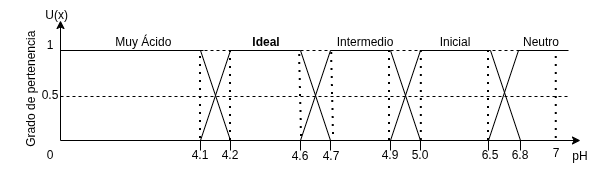
\includegraphics[width=1\textwidth]{./UML/Modulo2/diseno/logica1.drawio.png}
    \caption{Función de membresiá pH}
    \label{fig:Log1}
    \end{figure} 

    

\newpage

    De la misma manera se establecen los rangos de la temperatura y sus respectivas etiquetas 
lingüísticas en la tabla \cref{tab:dominio_temp} ,durante el proceso de fermentación del kéfir, misma que se diseño con base a los estudios propuestos por Fitrianingsih Fitrianingsih y colaboradores \cite{Fitrianingsih2022}.
Dichos dominios siguen la misma estructura de la fórmula \eqref{eq:trapezoidal}, 
por lo que se definen las funciones de pertenencia trapezoidales en la \cref{fig:Log2}.

\begin{table}[h!]
    \centering
    \caption{Dominio de Valores de Temperatura }
    \label{tab:dominio_temp}
    % Se mantiene la estructura centrada y flexible de tabularx
    \begin{tabularx}{\textwidth}{|>{\centering\arraybackslash}X|>{\centering\arraybackslash}X|>{\centering\arraybackslash}X|>{\centering\arraybackslash}X|>{\centering\arraybackslash}X|>{\centering\arraybackslash}X|}
        \hline
        % Cabecera superior: Se mantiene en 3 filas de alto
        \multirow{3}{*}{\textbf{Criterio}} & \multirow{3}{*}{\textbf{Etiqueta}} & \multicolumn{4}{c|}{\textbf{Dominio de Temperatura (x)}} \\ 
        \cline{3-6} 
    
        % Los multicols deben usar 'c' o un tipo de columna centrado.
        % NOTA: Se corrige la notación de dominio a su forma común
        & & \multicolumn{1}{c|}{\textbf{a < x < b}} & \multicolumn{2}{c|}{\textbf{b < x < c}} & \multicolumn{1}{c|}{\textbf{c < x < d}} \\ 
        \cline{3-6} 
        
        & & \textbf{a} & \textbf{b} & \textbf{c} & \textbf{d} \\ 
        \hline
        
        % Se ajusta \multirow a 5 filas para contener todos los nuevos datos
        \multirow{5}{*}{\textbf{Temp.}}
        & Muy frío & $0^\circ\text{C}$ & $2^\circ\text{C}$ & $10^\circ\text{C}$ & $12^\circ\text{C}$ \\ 
        \cline{2-6} 
        
        & Frío & $10^\circ\text{C}$ & $12^\circ\text{C}$ & $16^\circ\text{C}$ & $18^\circ\text{C}$ \\ 
        \cline{2-6} 
        
        & Ambiente & $16^\circ\text{C}$ & $18^\circ\text{C}$ & $25^\circ\text{C}$ & $27^\circ\text{C}$ \\ 
        \cline{2-6} 
        
        & Caliente & $25^\circ\text{C}$ & $27^\circ\text{C}$ & $30^\circ\text{C}$ & $32^\circ\text{C}$ \\ 
        \cline{2-6} 
        
        % La última fila fusiona las columnas y se corrige la notación
        & Muy Caliente & $30^\circ\text{C}$ & \multicolumn{3}{c|}{$\text{Temp.} \geq 32^\circ\text{C}$} \\ 
        \hline
    \end{tabularx}
\end{table}

 \begin{figure}[htb]
    \centering
    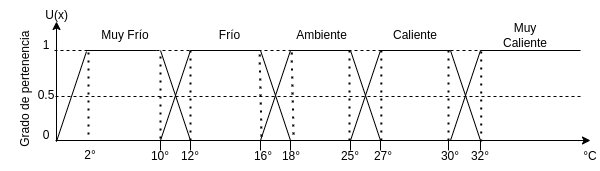
\includegraphics[width=.9\textwidth]{./UML/Modulo2/diseno/logica2.drawio.png}
    \caption{Función de membresiá Temperatura}
    \label{fig:Log2}
    \end{figure} 

\newpage 
A partir de lo anterior, se construye la matriz de reglas difusas presentada en la 
\cref{tab:reglas_ph_temp}, la cual integra las variables de entrada pH y 
temperatura para determinar la condición del kéfir en cada escenario posible para 
las categorías resultantes.Las cuales se detallan las reglas en el anexo A las reglas.


\begin{table}[h!]
    \centering
    \caption{Matriz de Reglas Difusas para la clasificación del kéfir.}
    \label{tab:reglas_ph_temp}
    
    % Ahora son 6 columnas
    \begin{tabularx}{\textwidth}{|X|X|X|X|X|X|}
        \hline
        
        % Fila 1
        \multirow{2}{*}{\textbf{Temp.}} & \multicolumn{5}{c|}{\textbf{pH}} \\
        \cline{2-6}
        
        % Fila 2
        & \textbf{Neutro} & \textbf{Inicial} & \textbf{Intermedio} & \textbf{Ideal} & \textbf{Muy Ácido} \\
        \hline
        
        % Filas de datos
        \textbf{Muy Frío} 
        & Inhibición (IN) 
        & Inhibición (IN) 
        & Inhibición (IN) 
        & Inhibición (IN) 
        & Riesgo Bajo (RIB) \\
        \hline
        
        \textbf{Frío} 
        & Deficiente (DEF)
        & Inicialmente Aceptable (IACE) 
        & Progresiva- mente Aceptable (PACE) 
        & Semi-Óptimo (SO) 
        & Sobreferme- ntado (SOB) \\
        \hline
        
        \textbf{Ambiente} 
        & Deficiente (DEF)
        & Inicialmente Estable (IES) 
        & Progresiva- mente Estable (PES) 
        & \textbf{Perfecto (PER)} 
        & Sobreferme- ntado (SOB) \\
        \hline
        
        \textbf{Caliente} 
        & Deficiente (DEF)
        & Inicialmente Aceptable (IACE) 
        & Progresiva- mente Aceptable (PACE) 
        & Semi-Óptimo (SO) 
        & Sobreferme- ntado (SOB) \\
        \hline
        
        \textbf{Muy Caliente} 
        & Peligro (PE)
        & Deficiente (DEF) 
        & Deficiente (DEF) 
        & Deficiente (DEF) 
        & Peligro (PE) \\ 
        \hline
    \end{tabularx}
\end{table}

\subsubsection{Salud de la fermentación}

Con base en el marco teórico desarrollado, la liberación de $\text{CO}_2$ durante la fermentación del
kéfir mantiene una relación inversamente proporcional con el pH indicando su salud. Este, a su vez, 
depende directamente de la temperatura, la cual ejerce un control decisivo sobre la cinética de 
ambos procesos, dado que estos compuestos son productos del metabolismo 
conjunto de las bacterias lácticas y levaduras presentes en los gránulos.

No obstante, la rapidez de esta liberación constituye un indicador crítico del estado de salud del 
cultivo. Cuando se emplea una alta concentración de gránulos en relación con un volumen reducido de leche, 
la producción de $\text{CO}_2$ se acelera de manera abrupta, generando condiciones de hipercarbonatación que 
comprometen el equilibrio organoléptico y la viabilidad probiótica del producto final, e incluso pueden 
derivar en una sobrefermentación. Por el contrario, una proporción escasa de 
gránulos genera niveles muy bajos de $\text{CO}_2$, lo que, aunque no compromete la salud de los microorganismos, 
prolonga considerablemente los tiempos de fermentación y retrasa la obtención de las características 
deseadas.

En consecuencia, la \cref{tab:dominio_co2} presenta los dominios difusos basados en la fórmula \eqref{eq:trapezoidal}, 
los cuales establecen cuatro etiquetas lingüísticas: Bajo, Medio, Alto y 
Excesivo (expresadas en ppm, unidad entregada directamente por el sensor). Estas se ilustran en la \cref{fig:Log3}.

\begin{table}[htbp]
    \centering
    \caption{Dominio de Valores de $CO_{2}$ por Etiqueta}
    \label{tab:dominio_co2}

 \begin{tabularx}{\textwidth}{|>{\centering\arraybackslash}X|>{\centering\arraybackslash}X|>{\centering\arraybackslash}X|>{\centering\arraybackslash}X|>{\centering\arraybackslash}X|>{\centering\arraybackslash}X|}
        \hline
        % Cabecera superior: Se mantiene en 3 filas de alto
        \multirow{3}{*}{\textbf{Criterio}} & \multirow{3}{*}{\textbf{Etiqueta}} & \multicolumn{4}{c|}{\textbf{Dominio de CO$_2$ (ppm)}} \\ 
        \cline{3-6} 
        & & \multicolumn{1}{c|}{\textbf{a < x < b}} & \multicolumn{2}{c|}{\textbf{b < x < c}} & \multicolumn{1}{c|}{\textbf{c < x < d}} \\ 
        \cline{3-6} 

    & & \textbf{a} & \textbf{b} & \textbf{c} & \textbf{d} \\
    \hline
    \multirow{5}{*}{\textbf{CO$_2$}}
    & Muy Bajo      & 0     & 0     & 400   & 500  \\ \cline{2-6}
    & Bajo     & 400  & 500  & 1200  & 1300 \\ \cline{2-6}
    & Media     & 1200  & 1300  & 2000  & 2100  \\ \cline{2-6}
    & Alto      & 2000  & 2100  & 3200  & 3300  \\ \cline{2-6}
    & Excesivo  & 3200  &  \multicolumn{3}{c|}{$\text{$CO_{2}$} > 3300$}  \\ \hline
    \end{tabularx}
\end{table}


 \begin{figure}[htbp]
    \centering
    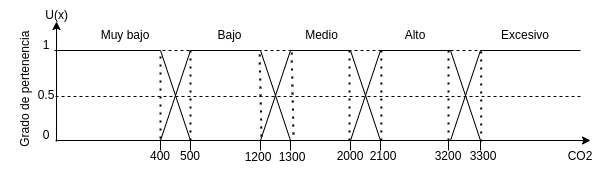
\includegraphics[width=.9\textwidth]{./UML/Modulo2/diseno/logica3.drawio.png}
    \caption{Función de membresá $CO_{2}$}
    \label{fig:Log3}
    \end{figure} 

Para la clasificación del estado de la fermentación, se construye la matriz de reglas difusas 
presentada en la \cref{tab:reglas_co2_ph},
la cual integra las variables de entrada pH y concentración de $CO_{2}$ para determinar la condición 
del kéfir en cada escenario posible, asimismo en el anexo A se detallan las reglas en la lista.
\begin{table}[htbp]
    \centering
    \caption{Matriz de Reglas Difusas para la salud del kéfir .}
    \label{tab:reglas_co2_ph}
    
    \begin{tabularx}{\textwidth}{|>{\centering\arraybackslash}X|>{\centering\arraybackslash}X|>{\centering\arraybackslash}X|>{\centering\arraybackslash}X|>{\centering\arraybackslash}X|>{\centering\arraybackslash}X|}
        \hline
        
        \multirow{2}{*}{\textbf{CO$_2$}} & \multicolumn{5}{c|}{\textbf{pH}} \\
        \cline{2-6}
        
        & \textbf{Neutro} & \textbf{Inicial} & \textbf{Intermedio} & \textbf{Óptimo} & \textbf{Ácido} \\
        \hline
        
        \textbf{Muy Bajo} 
        & Inactivo (INA) 
        & Inactivo (INA) 
        & Inactivo (INA) 
        & Inactivo (INA) 
        & Inestable (INE) \\
        \hline
        
        \textbf{Bajo} 
        & Inactivo (INA) 
        & Saludable (SAL) 
        & Saludable (SAL) 
        & Saludable (SAL) 
        & Excesivo (EXC) \\
        \hline
        
        \textbf{Media} 
        & Inestable (INE) 
        & Saludable (SAL) 
        & Saludable (SAL) 
        & \textbf{Óptimo (OPT)} 
        & Excesivo (EXC) \\
        \hline
        
        \textbf{Alto} 
        & Riesgo (RIE) 
        & Saludable (SAL) 
        & Saludable (SAL) 
        & \textbf{Óptimo (OPT)} 
        & Excesivo (EXC) \\
        \hline
        
        \textbf{Excesivo} 
        & Riesgo (RIE) 
        & Excesivo (EXC) 
        & Excesivo (EXC) 
        & Excesivo (EXC) 
        & Riesgo (RIE) \\ 
        \hline
    \end{tabularx}
\end{table}

\newpage

\subsubsection{Estado de la fermentación}

Con base en los resultados de ambas matrices, se determina 
el estado de la fermentación en cada escenario operativo 
mediante una tercera matriz de evaluación, la cual consolida de 
manera exclusiva las salidas de las dos fases anteriores, 
tal como se ilustra en la \cref{tab:matriz_evaluadora_final}. 
Este esquema implementa un enfoque híbrido entre el modelo de inferencia de
Mamdani y una clasificación lingüística experimental, 
transformando los valores cuantitativos obtenidos de ambos modelos 
en un diagnóstico cualitativo unificado. Asimismo, la arquitectura general 
de este modelo se presenta en la \cref{fig:Cir1}.

Asimismo, en la \cref{tab:explicacion_etiquetas_globales} ubicada en el Anexo se incluye una tabla detallada
que explica cada una de las categorías resultantes, 
junto con sus implicaciones prácticas para la toma de decisiones durante la producción del kéfir.

\begin{table}[htbp]
    \centering
    \caption{Matriz Evaluadora Final para el Diagnóstico Global del Kéfir.}
    \label{tab:matriz_evaluadora_final}
    
    \begin{tabularx}{\textwidth}{|>{\centering\arraybackslash}X|>{\centering\arraybackslash}X|>{\centering\arraybackslash}X|>{\centering\arraybackslash}X|>{\centering\arraybackslash}X|>{\centering\arraybackslash}X|}
        \hline
        
        \multirow{2}{*}{\textbf{Acidificación}} & \multicolumn{5}{c|}{\textbf{Salud}} \\
        \cline{2-6}
        
        & \textbf{Inactiva (INA)} & \textbf{Lenta / Inicial} & \textbf{Progresiva / Mod.} & \textbf{Óptima (OPT)} & \textbf{Hipercarb. / RIE} \\
        \hline
        
        \textbf{Inhibición (IN)} 
        & Caduco (CAD) 
        & Incompleto (INC) 
        & Incompleto (INC) 
        & Riesgo (RIE) 
        & Peligro (PEL) \\
        \hline
        
        \textbf{Deficiente (DEF)} 
        & Caduco (CAD) 
        & Incompleto (INC) 
        & Aceptable (ACE) 
        & Aceptable (ACE) 
        & Riesgo (RIE) \\
        \hline
        
        \textbf{Aceptable / Estable} 
        & Incompleto (INC) 
        & Aceptable (ACE) 
        & Aceptable (ACE) 
        & Óptimo (OPT) 
        & Riesgo (RIE) \\
        \hline
        
        \textbf{Perfecto / Semi-Ópt.} 
        & Incompleto (INC) 
        & Aceptable (ACE) 
        & Óptimo (OPT) 
        & \textbf{Perfecto (PER)} 
        & Riesgo (RIE) \\
        \hline
        
        \textbf{Sobreferm. / Peligro} 
        & Peligro (PEL) 
        & Riesgo (RIE) 
        & Riesgo (RIE) 
        & Riesgo (RIE) 
        & Peligro (PEL) \\ 
        \hline
    \end{tabularx}
\end{table}

\begin{figure}[htb]
    \centering
    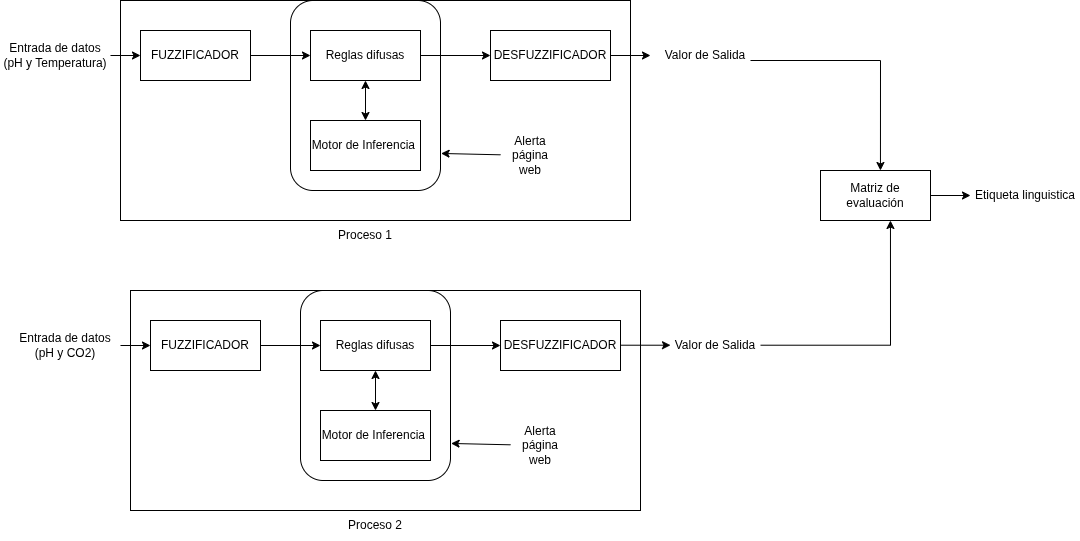
\includegraphics[
        width=1\textwidth,        % Máximo ancho del texto disponible
        height=1\textheight,  % Máximo alto del texto (usamos 95% para dejar espacio al pie)
        keepaspectratio          % Mantiene las proporciones originales
    ]{./UML/Modulo2/diseno/logicacascada.drawio.png}
    \caption{Circuito eléctrico del módulo 1}
    \label{fig:Cir1}
\end{figure}